\documentclass{pjsivi}

% \usepackage[francais]{babel}
% \usepackage[T1]{fontenc}
% \usepackage{graphicx}
% \usepackage{apalike}
% \usepackage{setspace}
% \usepackage{cite}
% \usepackage[utf8]{inputenc}
% \usepackage{color}
% \usepackage{multicol}
% \usepackage{setspace}

\usepackage[utf8]{inputenc}
\usepackage[T1]{fontenc}
\usepackage[francais]{babel}

%couleur
\usepackage{color}
\usepackage{multicol}

\usepackage{setspace}

%image
\usepackage{graphicx}

% code color

\definecolor{ligthyellow}{RGB}{250,247,220}
\definecolor{darkblue}{RGB}{5,10,85}
\definecolor{ligthblue}{RGB}{1,147,128}
\definecolor{darkgreen}{RGB}{8,120,51}
\definecolor{darkred}{RGB}{160,0,0}
\definecolor{univ}{RGB}{177,23,119}
\definecolor{univmodif}{RGB}{148,74,120}
\definecolor{mygray}{RGB}{100,100,100}


\hypersetup{       % parametrage des hyperliens
  colorlinks=true,  % colorise les liens
  breaklinks=true,  % permet les retours à la ligne pour les liens 
                    % trop longs
  urlcolor= blue,   % couleur des hyperliens
  linkcolor= black, % couleur des liens internes aux documents 
                    % (index, figures, tableaux, equations,...)
  citecolor= univ   % couleur des liens vers les references 
                    % bibliographiques
}


%TODO revoir le titre ce n'est plus juste un état de l'art

\begin{document}

%% PAGE DE GARDE
%% =============

\ 
\vspace{1cm}

\begin{multicols}{2}  

    \textbf{\large Auteurs:}
    \begin{itemize}
      \item Alexis ROBACHE
      \item Elliot VANEGUE
      \item Gaëtan DEFLANDRE
    \end{itemize}
    
    \textbf{\large Encadrants:}\\
    \begin{itemize}
      \item Hazem WANNOUS
      \item Jean-Philippe VANDEBORRE 
    \end{itemize}

\end{multicols}

\vspace{4cm}

 \begin{flushright}
  \begin{spacing}{1.6}
    \textbf{
      {\LARGE Présentation et état de l'art sur la détection, 
      le suivi de la main et animation de celle-ci dans une scène 3D}
    }
  \end{spacing}
  \hrule
  \vspace{0.2cm}
  \textit{
    {\Large\textcolor{mygray}{Projet \og Hand Kinect \fg, Master IVI}}
  }
\end{flushright}

\vspace{4cm}

\begin{center}
  
\includegraphics[height=3.5cm]{images/logoLILLE1.jpg}
  \hfill
  % logo équipe
  %\includegraphics[height=3.5cm]{image/}
  \vspace{4cm}


  {\large\textbf{Octobre 2015 à Février 2016}}
\end{center}



\newpage



%% TABLE DES MATIERES
%% ==================

\tableofcontents

\newpage



%% RESUME
%% ======

%% vraiment à mettre pour un edla ?

%\begin{abstract}
%TODO
%\end{abstract}

%\newpage



%% INTRO
%% =====

\section{Introduction}

Durant notre master IVI\footnote{Le master Image Vision Interaction est 
l'un des parcours des masters informatiques de l'université de Lille 1}, 
nous avons l'occasion de réaliser un projet orienté recherche. Nous avons 
sélectionné le sujet \og Hand Kinect \fg, car nous nous intéressons à la 
modélisation 3D et aux dernières techniques d'acquisition.



\newpage



%% DEVELOPPEMENT
%% =============

\chapter{Présentation générale}



%doit contenir la fonction de ce rapport : etat de l'art + previsionnel
%dans le but de réaliser un projet
\section{Présentation du projet}
Aujourd'hui, détecter les points des articulations du corps humain 
est une technique courante, grâce à certain périphérique tel que la 
Kinect. Les points des articulations du corps forment le squelette 3D. 
Cependant, les squelettes 3D sont en générales peu riche en informations 
concernant les points des articulations des mains.\\
 
Pourtant les mains sont habiles et nous pouvons faire de nombreux 
mouvements, plus ou moins complexes et rapides avec elles. De plus en 
plus d'application nécessite des IHM plus précisent et plus 
naturelles. Utiliser ces mains pour contrôler, interagir et communiquer 
avec un ordinateur, devient de plus en plus intéressant. Ce niveau de 
précision peut être utile dans divers domains :
\begin{itemize}
  \item simulation médicale.
  \item modélisation et CAO.
  \item manipulation d'objets 3D virtuels.
  \item jeux vidéo.\\
\end{itemize}

Le projet \og Hand Kinect \fg consiste à extraire depuis une Kinect 2, 
les points correspondants aux articulations du corps grâce aux 
fonctions du SDK de Kinect. De plus, nous devons récupérer les points 
des articulations des mains, nous disposons d'un module fourni par 
nos tuteurs de projet. Ainsi, l'assemblage de ces points nous permet 
d'obtenir le squelette 3D complet de la personne devant la Kinect.\\

\begin{figure}[H]
  \begin{center}
    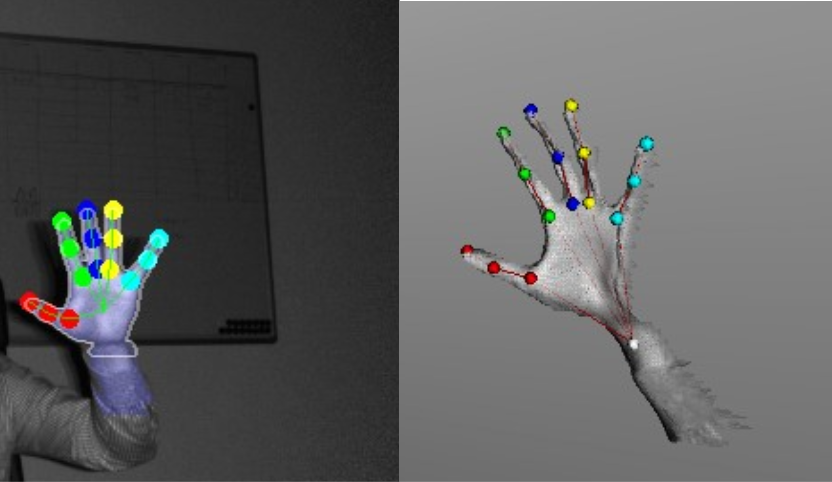
\includegraphics[width=350px]{images/joint_detection.png}
    \caption{Détection des articulations des mains}
  \end{center}
\end{figure}

Ensuite, nous souhaitons animer un modèle 3D, qui peut être un modèle 
d'humain, de robot ou bien de créature. Les mouvement de ce modèle 
doivent suivre les points du squelette préalablement détecté, de 
manière cohérente par rapport au mouvement de la personne devant la 
Kinect. Nous utilisons Unity3D, pour cette partie de 
modélisation.\\

Unity3D est un moteur de jeu qui permet de développé rapidement des 
environnement et application 3D. Il est facile d'obtenir des 
application compatible sur de nombreuse plateforme. Ce moteur 
propose également une licence gratuit accés compléte.\\

\begin{figure}[H]
  \begin{center}
    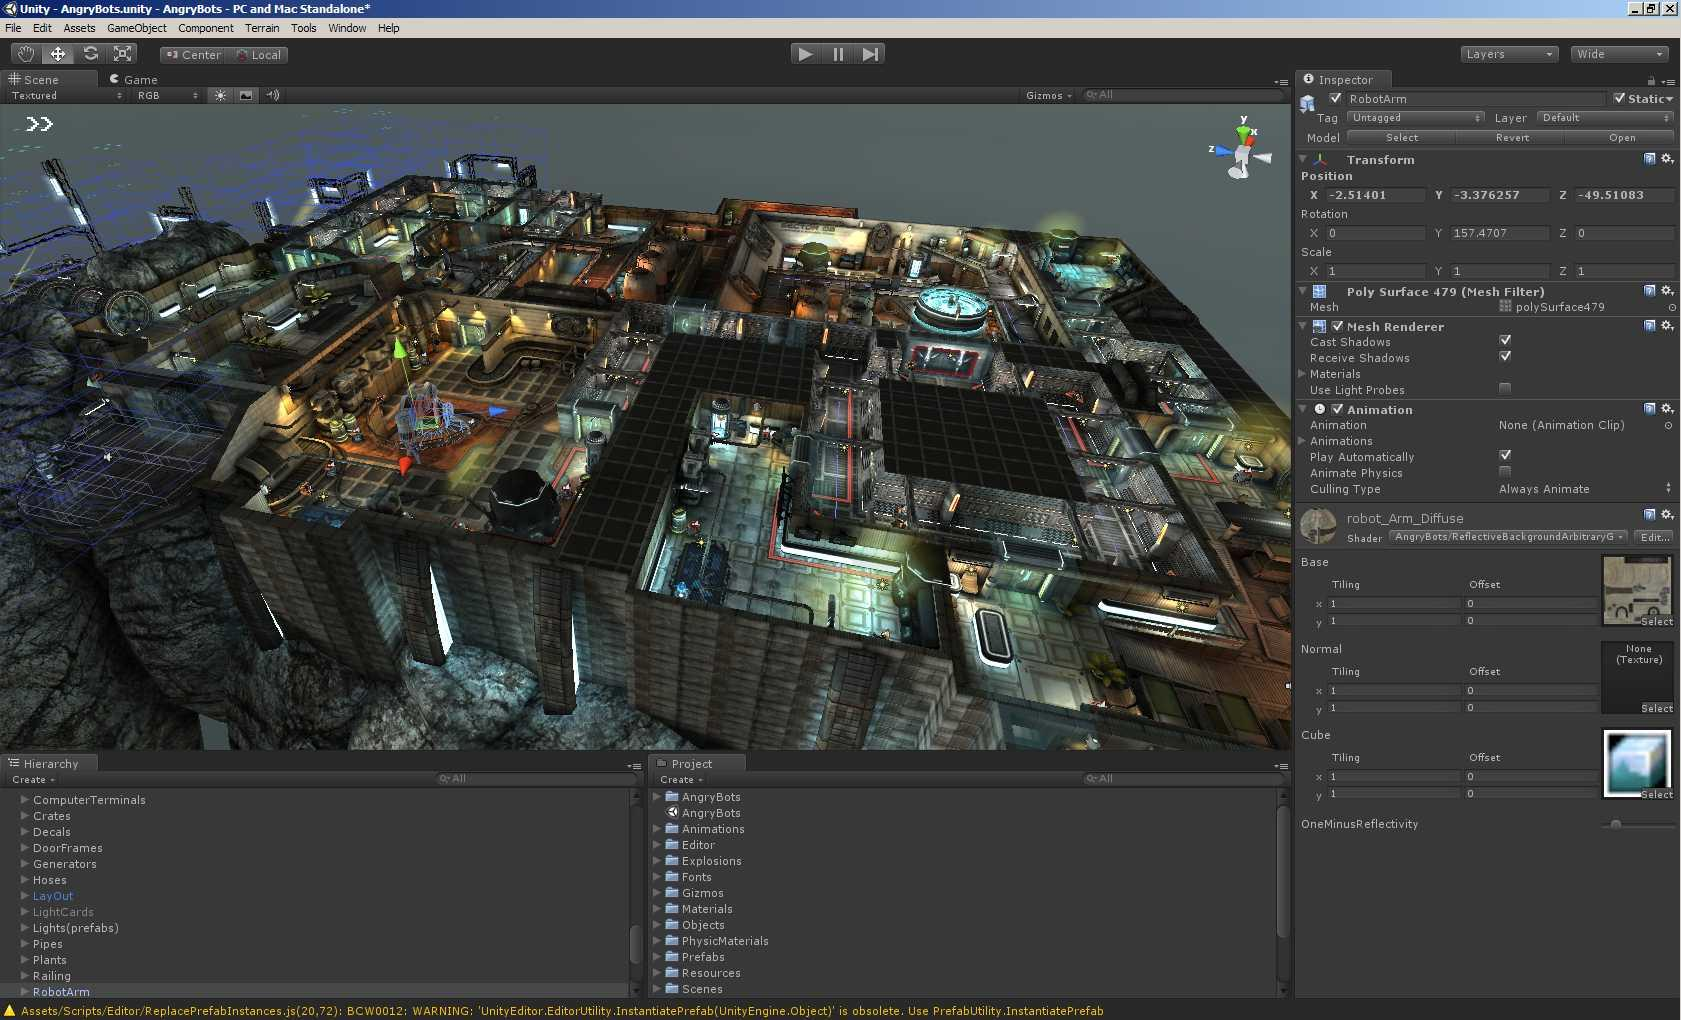
\includegraphics[width=350px]{images/Unity3D.jpg}
    \caption{Interface de Unity3D}
  \end{center}
\end{figure}

Dans le cadre de ce projet, nous sommes amené à rédiger un état de la 
l'art. Cette première partie, nous permet de synthétiser et sélectionner 
les solutions. Notre objectif étant de détecter la main et les 
articulations de la main d'une personne, afin de modéliser en 3D la main 
de cette personne, dans des plans de caméra global ou rapprocher. Cela 
doit être réalisable en temps réel et à partir d'une caméra nous 
fournissant une image RGB et une image contenant l'information de 
profondeur de la scène filmée.\\

%doit contenir l'ensemble des informations sur l'équipe -> sur quoi porte leur recherche
\section{Contexte}
La réalisation de ce projet se fait avec l'équipe 3D 
SAM\footnote{Modeling and Analysis of Static and Dynamic Shapes}. 
Cette équipe appartient au centre CRIStAL\footnote{Centre de Recherche 
en Informatique, Signal et Automatique de Lille}. Ce centre de 
recherche est le nouveau pôle de recherche qui regroupe les 
laboratoires d'Informatique, Signal et Automatique de Lille.\\


L'équipe 3D SAM est basée à l'école d'ingénieur Télécom Lille 1. 
Cette équipe conçoit de nouveaux outils et méthodes d'analyse des 
formes des objets 3D statiques et dynamique. Ils travaillent sur 
l'analyse de formes des objects 3D et la modélisation des variations 
des formes dans des vidéos 3D.

\begin{figure}[H]
  \begin{center}
    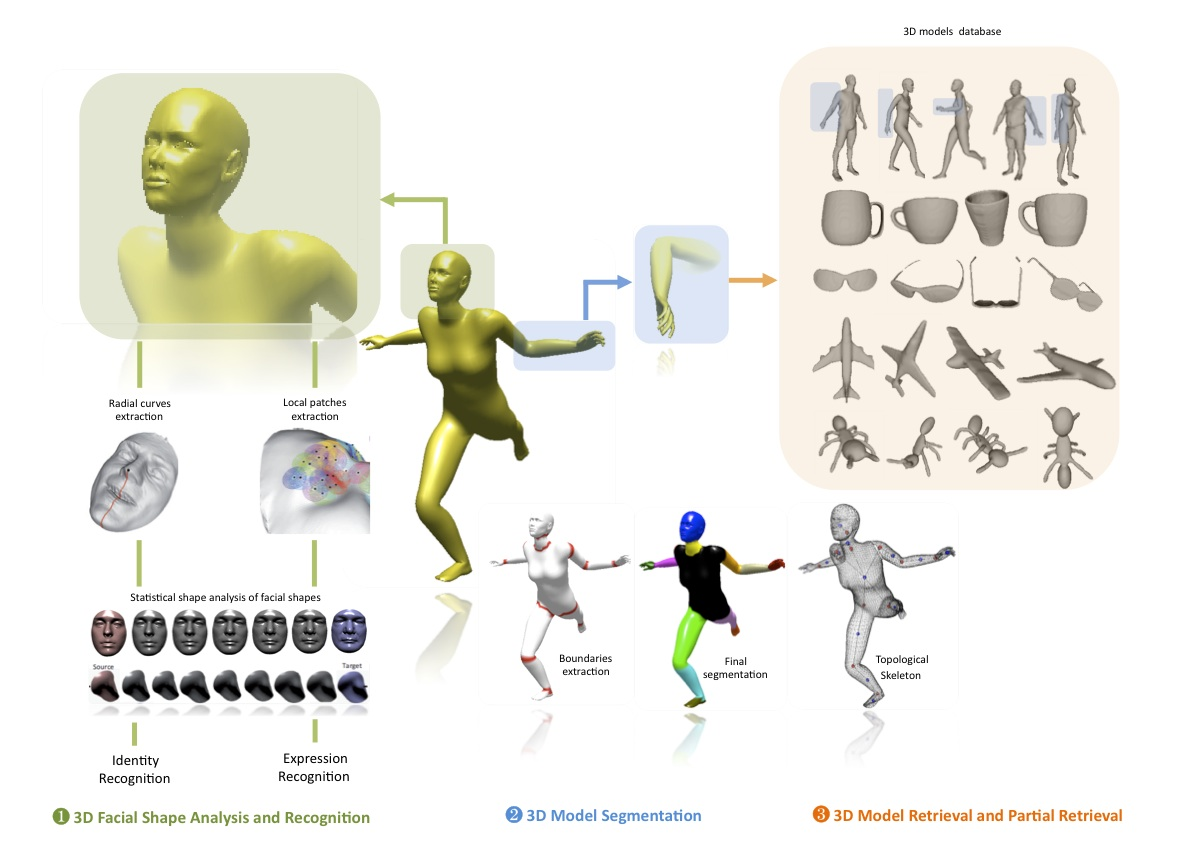
\includegraphics[width=300px]{images/accueil-illus.jpg}
    \caption{Exemples de travaux de l'équipe 3D SAM}
  \end{center}
\end{figure}

Le projet \og Hand Kinect \fg est un nouveau projet proposé par 
l'équipe. Nous sommes les premiers à travailler sur ce projet, il 
ne s'agit pas d'une reprise d'un projet déjà entamé auparavant.\\

Pour la réalisation de ce projet, nous disposons d'une caméra Kinect2. 
Pour les représentation et animation 3D, il nous faut un environnement 
de modélisation 3D, nous utilisons Unity3D comme montré précédemment. 
Nous disposons également, d'un module nous permettant d'extraire les 
points des articulation de la main.

%pourquoi faire ce projet (plus de precision?) + cas concret ou on pourrait l'utiliser (ex : medecine)
\section{Problèmatique}
D'abord, la Kinect 2 peux déjà de suivre 6 personne à la fois. Elle 
détecte un squelette de 25 points (voir Fig. 
\ref{fig:skeleton_kinect2}). Cependant, les mains ne sont représentées 
que par 3 point, qui sont le centre de main, le pouce et le bout du 
majeur. C'est une amélioration par rapport à la Kinect 1, qui de 
détecter que le centre de la main.\\

%a revoir
D'autre outils permettent de détecter les mains des utilisateurs. Par exemple le Leap Motion détecte les articulations des mains. Néanmoins,
ce capteur est limité car il faut garder les mains proches et dans le 
cadre du capture. Leap Motion ne permet pas de détecter le squelette 
d'une personne.\\

%a revoir
À partir de ces constats nous pouvons formuler la problèmatique 
suivante. Puisque, 
les mains sont très habile, il peut être difficile de detecter de leurs 
articulations dans des positions contraignante. Autres choses, les 
problèmes liés à la luminausitée sont récurrents, il est souhaitable 
d'utiliser des techniques robustent et invariantent à la luminausitée, 
mais qui restent efficace. De plus, il existe encore peu de méthodes 
permettant de détecter la pose et les articulations des mains dans 
un point de vue de caméra qui permetterais de retrouver l'ensemble du
squelette humain.  

%comment réaliser ce projet, avec quoi + résultat attendu
\section{Objectif}
L'objectif de notre projet est d'utiliser la Kinect 2 dans le but de détecter les différentes articulations
de la main et de modéliser celle-ci dans une application Unity.
%TODO ajouter les différentes étape de nos recherches 

\section{Présentation de la Kinect 2}
La Kinect 2 de Microsoft possède une caméra couleur en mode YUV de 1920x1080 pixel.
YUV est une combination particulière d'information pour restituer la couleur, comme RGB ou HSP.
Cette combinaison aussi appelée YCbCr, avec Y la luminance, U/Cb la composante bleu sans luminance et V/Cr la composante rouge sans luminance
En plus de sa caméra, elle possède 3 diffuseur de rayonnement infrarouges qui servent à dessiner une carte de profondeur.
Les autres fonctionnalités ne nous intéresseront pas résoudre notre problèmatique.\\

\begin{figure}[H]
 \center
 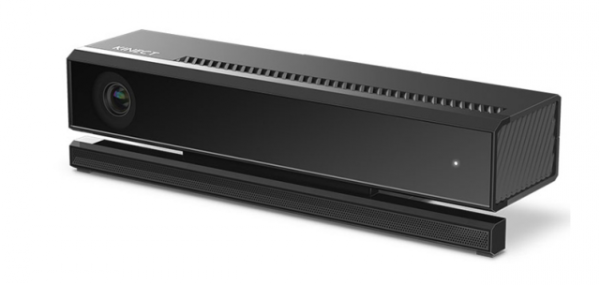
\includegraphics[width=300px]{images/kinect-v2.png}
 \caption{Caméra Kinect 2}
\end{figure}

On récupère donc de Kinect les données brutes suivantes : 
\begin{itemize}
 \item un flux vidéo couleur en YUV
 \item un flux vidéo d'images de profondeur
\end{itemize}

Ces deux flux peuvent servir à détecter la main (méthodes expliquées dans la partie état de l'art).
Le SDK de la Kinect fournit des informations déjà traitées. 
Par exemple pour notre projet, les jointures du poignet, du centre de la main, du sommet du pouce et du sommet du majeur.

\begin{figure}[H]
\center
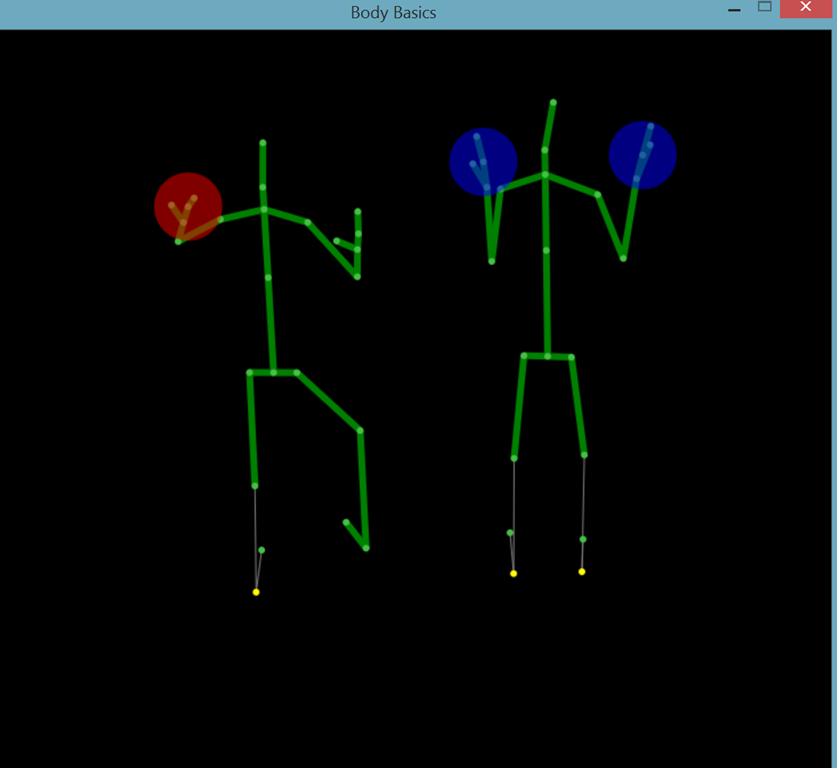
\includegraphics[width=250px]{images/kinec2_skel.png}
\caption{Squelette de l'utilisateur détecté par la Kinect 2}
\label{fig:skeleton_kinect2}
\end{figure}

%présentation du materiel + image materiel
%présentation des données brut
%présentation du sdk + image squelette

\chapter{Etat de l'art}

\section{Différents type de données}
Pour réaliser notre projet : animer un modèle de main en se basant sur les mouvements de la main de l'utilisateur, nous avons à disposition une 
Kinect 2 et un LeapMotion. Pour commencer notre état de l'art, nous allons voir quelles données peuvent être récupérées par ces outils et 
quels autres moyens auraient pu être utilisés pour réaliser ce projet.\\

Une liste non exhaustive des périphériques et des données utile qu'ils fournissent : 
\begin{itemize}
  \item Kinect et Kinect 2 de Microsoft, fournissent en données brutes une image couleur ainsi qu'une image de profondeur. 
En utilisant le SDK fournis, on dispose en plus de nombreux outils parmi lesquels une détection du squelette et pour Kinect 2 
une abstraction de la main avec 4 points détectés : le centre du poignet, le centre de la main, le sommet de pouce et le sommet du majeur. 
  \item LeapMotion et LeapMotion 2, fournissent en données brutes une image de profondeur plus détaillée mais sur une zone 
plus restreinte. Avec le SDK, on a accès directement à un squelette très détaillé de la main.
    \begin{figure}[!h]
    \center
    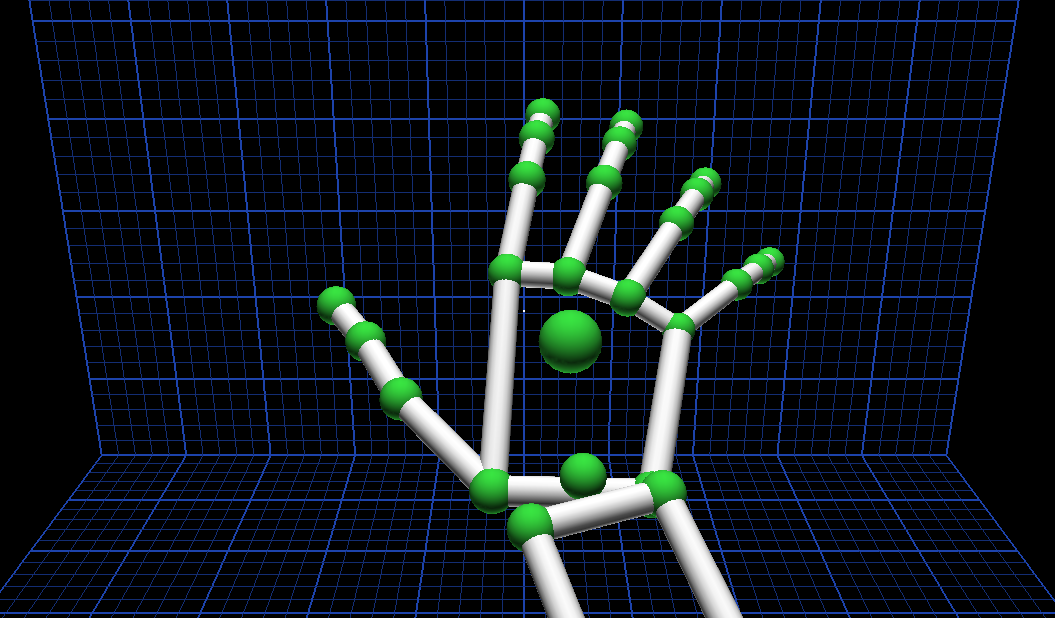
\includegraphics[width=350px]{images/SDK_LeapMotion.png}
    \caption{Squelette de la main de l'utilisateur détecté par la LeapMotion}
    \end{figure}
  \item RealSense est un périphérique relativement récent, à mis chemin entre Kinect 2 et LeapMotion. On peut, à l'aide du SDK fournis, récupérer des informations semblables à celles fournies par LeapMotion : 
  22 points de la main détectés et suivits
\end{itemize}
\ \\

On peut utiliser des outils spécifiques (Kinect) ou des caméras classiques pour obtenir des images couleurs.
Bien que possédant plus d'informations que les images de profondeur (3 canaux au lieu d'1), les images couleurs ne sont pas adaptées à la détection de la position dans l'espace (pas de données 3D).\\
Ces données couleurs peuvent être utilisées avec des accessoires colorés pour simplifier la détection des points de la main. \cite{wang2009real}
Cette méthode permet de détecter plus facilement les jointures et les points d'intér\^{e}t. 
Cependant, cela ajoute des contraintes, notemment le fait de devoir porter un gant standardisé.\\

On associe également les données couleurs avec des données de profondeur pour améliorer la détection et gérer les cas de superposition. \cite{van2011combining}\\

L'autre type de données est la carte de profondeur, image en niveau de gris servant à représenter la profondeur. 
Cette carte de profondeur est utilisée par un grand nombre de méthodes pour les problèmes de clustering du corps humain, notemment les SDK de Kinect et Kinect 2 se base principalement dessus pour fournir le squelette.\cite{export:145347}
Les SDK de Kinect/Kinect2 étant prévus pour le suivit du corps entier, il sont peu performant pour le suivit précis de parties spécifique (comme la main).
L'utilisation directe du SDK semble dont insufisante pour résoudre notre problème. Cependant, on peut aussi récupérer les données brutes fournies par la Kinect 2 et certaines méthodes se contentent d'une image de profondeur pour la détection de la main. \cite{export:238453}

\section{Détection de la main}

La Kinect possède deux types de caméra, une caméra couleur et une caméra de profondeur utilisant la méthode 
\og Time of Flight \fg. Les caméras de type \og Time of Flight \fg envoient des rayons infrarouges. Une caméra infrarouge
récupére ensuite les rayons réfléchit, ce qui permet d'obtenir les informations de profondeur. 
Il existe plusieurs solutions utilisant l'une ou l'autre de ces caméras. Nous allons
dans cette partie détailler plusieurs méthodes réalisées jusqu'à maintenant.

\subsection{Détection et suivi de la main à partir d'une image couleur}
La méthode proposée par S. Bilal et al \cite{haarlike} utilise l'algorithme de Viola et al \cite{viola2001jones} afin
de détecter la main et fournir la position de celle-ci en créant une ROI\footnote{Region Of Interest} autour d'elle.
L'algorithme de Viola et al \cite{viola2001jones} nécessite une 
base de connaissances composée des caractéristiques de l'objet recherché. Elle est utilisée dans un 
apprentissage supervisé, c'est-à-dire que l'algorithme a besoin de données représentant
l'objet à détecter pour classifier les caractéristiques de celui-ci. Cet algorithme est basé sur des caractéristiques 
pseudo-Haar qui crée des masques rectangulaires et adjacents dans différentes zones de l'image (voir Fig. \ref{fig:pseudo_haar}). 
Chaque masque calcule l'intensité des pixels qu'il contient, puis l'algorithme fait la différence entre les masques blancs et 
les masques noirs.\\

\begin{figure}[!h]
\center

\includegraphics[width=200px]{images/pseudo_haar.png}
\caption{Exemple de caractéristiques pseudo-Haar utilisées pour l'algorithme Viola et Jones}
\label{fig:pseudo_haar}
\end{figure}

Pour améliorer les perfomances de leur algorithme, Viola et Jones utilisent la méthode Adaboost. Son
principe est de sélectionner les caractéristiques les plus performantes pour la détection de l'objet grâce à
un calcul de probabilité utilisant l'entropie\footnote{valeur mesurant l'incertitude d'une donnée} des données.\\

Une fois, qu'une ROI est formée autour de la main de l'utilisateur S. Bilal et al \cite{haarlike} changent d'espace colorimétrique
afin de pouvoir différencier la main du reste de l'environnement. Pour cela, ils choisissent 
d'utiliser l'espace YCbCr qui permet d'obtenir des informations de chromaticité dont la valeur est presque équivalente
quelle que soit la couleur de peau de l'utilisateur \cite{yoo1999fast}. Une fois que la ROI de la main est binarisé, il est possible
de détecter le bout des doigts. Il faut tout d'abord calculer le centroïde de la forme de la main, puis la distance entre
ce centroïde et chaque point du contour de la main. Le contour d'une forme dans une image est défini par un changement brutal
de couleur. Cette méthode permet d'obtenir un graphe correspondant à la Fig. \ref{fig:handHisto}, où chaque pique représente un doigt.

\begin{figure}[!h]
\center
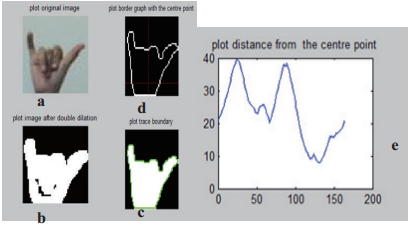
\includegraphics[width=300px]{images/handHisto.png}
\caption{Histogramme des distances entre les points du contour de la main et le centroide}
\label{fig:handHisto}
\end{figure}

\newpage

Afin de pouvoir traquer la main, S. Bilal et al \cite{haarlike} utilisent l'algorithme de Kalman \cite{kalman}.
Cet algorithme permet de prédire la position d'un objet, ce qui va permettre de traquer la main malgré
le bruit présent dans l'image. De plus, cette méthode n'a besoin de connaître que l'état précédent à celui 
qui est calculé. Etant donné que l'algorithme de Kalman est un algorithme de prédiction, il peut ne pas être très
précis lorsque l'utilisateur effectue des changements de direction rapides avec sa main.\\

Cette méthode, nous permet de déterminer la position de la main et de détecter le bout des doigts. Cependant, elle ne nous permet
pas de réaliser notre projet entièrement. En effet, nous avons besoin de plus de précision en détectant les articulations
de la main. De plus, cette méthode est sensible à la luminosité de la scène filmé et n'est pas très adapté
à la modélisation 3D d'une main.

\subsection{Détection et suivi de la main avec une image de profondeur}
Une seconde solution utilise une image de profondeur plutôt que l'image binarisée avec le changement d'espace colorimétrique.
Pour réaliser la détection de la main, il faut dans un premier temps déterminer une ROI
autour de celle-ci. Cette première étape a été expliquée par T. Sharp et al\cite{export:238453}, où les auteurs utilisent un classifieur
qui se repose sur la méthode développée dans \cite{export:145347}. Ce classifieur permet d'effectuer de la reconnaissance
des parties du corps et permet également de détecter les articulations. Pour cela, cette méthode utilise l'algorithme \cite{lepetit2005randomized} qui crée un arbre de décision partir des données d'entrainement et descend dans celui-ci
jusqu'à atteindre une feuille. 
Les feuilles de cet arbre sont les différentes parties du corps à reconnaître. Cet arbre est construit en calculant
l'entropie de chaque pixel, ce qui permet de déterminer à quelle partie du corps il appartient.

\begin{figure}[!h]
 \begin{center}
  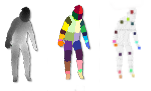
\includegraphics[width=300px]{images/bodyrecognition.png}
  \caption{Résultat de la détection des parties du corps et des articulations grâce à la méthode de \cite{export:145347}}
  \label{fig:bodyrecognition}
 \end{center}
\end{figure}

On voit sur la Fig. \ref{fig:bodyrecognition} que l'articulation de la main est détectée, il est alors possible de construire
une ROI autour de ce point. Cette méthode a été implémentée dans la caméra Kinect.\\

La méthode utilisée dans \cite{export:238453} ne nécessite aucune donnée provenant d'image antérieure. L'ensemble
des calculs sont réalisés sur une image à partir d'une base de connaissances contenant différentes postures de la
main. Etant donnée qu'il est impossible de stocker toutes les postures de la main, la méthode de \cite{export:238453}
calcule une fonction energy permettant de déterminer quelle est la posture la plus représentative de celle de la main
de l'utilisateur. Cette fonction energy est calculée à partir des pixels du modèle et ceux de l'image de profondeur
capturée par la caméra. Elle est définie par le calcul suivant :
\begin{equation}
 E^{au}(Z_{roi}, R_{roi}) = \sum_{ij} \bar{\rho(z_{ij}} - r_{ij})
\end{equation}
Dans cette équation, $z_{ij}$ représente le pixel à la position (i,j) dans le modèle et $r_{ij}$ représente le pixel à la position (i,j)
provenant de l'image de profondeur. La fonction $\rho(e)$ quant à elle est équivalente à $min(|e|,\tau)$ ou $\tau$ est une valeur fixe permettant d'éliminer le bruit présent dans l'image de profondeur.

\section{Modélisation de la main}
%input
Pour mieux visualiser les actions réalisées par la main de l'utilisateur et pour faire correspondre les jointures détectées au modèle, il est nécessaire d'avoir
un modèle de la main qui soit réaliste et précis par rapport à la réalité. Pour cela, nous avons besoin d'un
mesh d'une main modèle que nous allons ensuite adapté à la main de l'utilisateur.\\

%icp
La méthode utilisé par \cite{export:217428} permet en utilisant l'algorithme
ICP\footnote{Iterated Closest Point} \cite{121791} de modifier le mesh de la main afin
que les points de celui-ci aient une distance moins importante avec le nuage de point fourni pas la 
caméra. Pour cela, l'algorithme ICP recherche les transformations, rotation et translation, qui permettent 
à partir d'un mesh M d'obtenir un mesh P. Dans notre cas, le mesh M représente le modèle de main donné en entré
et le mesh P représente la main de l'utilisateur. ICP fonctionne en quatre étape distincte.
\begin{itemize}
  \item On associe les points grâce aux critères du plus proche voisin. Pour cela, il suffit de calculer la distance euclidienne d'un
   point avec tous les autres points qui font parti du balayage que nous voulons comparer et de prendre la distance la plus petite.
  \item On estime la transformation des points grâce à une fonction d'erreur quadratique moyenne, permettant ainsi de trouver la meilleure
  transformation possible.
  \item On effectue la transformation du nuage de point ayant la plus petite erreur.
  \item On itere jusqu'à ce qu'on est atteint la condition de fin fixé par l'utilisateur.
\end{itemize} 
\ \\

%squelette
La méthode de \cite{export:217428} permet également d'adapter le squelette du modèle de la 
main, ce qui permet d'obtenir une précision plus importante lors de l'utilisation de l'application.
Pour cela, on applique à chaque os du squelette du model d'origine, 
une transformation ( rotation et forme) qui dépend de celle calculée par la phase précédente.\\

%Surface
Ensuite, la méthode recalcule la surface à partir du nouveaux mesh et du nouveau squelette.
Si la surface est paramétrée par un ensemble de points de controle, comme un polyèdre
ou une surface de subdivision, on applique une fonction surface pour retrouver le point de l'espace
correspondant.
Si le mesh est composé de triangles, on exprime le point de l'espace en u,v par une interpolation linéaire
entre les sommets du triangles correspondant.\\

%Optimisation
Entre chaque opération, on applique une fonction de minimisation d'énergie,
on obtient alors une convergence des résultats plus rapide qu'en utilisant simplement ICP une fois.

\section{Evaluation des solutions envisagées}
Parmi les solutions que nous avons envisagées dans cet état de l'art, nous avons vu que la solution avec une 
image couleur pouvait être limitée. Celle-ci nécessite un algorithme de tracking permettant de suivre au mieux
la main de l'utilisateur. L'algorithme de Kalman est efficace, mais peu précis lors de changements d'orientation
brusques et il est également assez complexe à mettre en place.\\

Notre choix pour la réalisation de ce projet se dirige plutôt vers l'utilisation de la caméra de profondeur.
La Kinect ayant déjà une implémentation d'une partie des étapes permettant la réalisation de notre projet, nous pourrons
nous concentrer sur la partie plus spécifique de détection et de localisation des articulations de la main. 
Pour cela, nous avons vu que la méthode utilisant l'image de profondeur pouvait être efficace grâce à la 
détermination de la posture de la main. Cela nous permet ainsi d'ajuster un modèle de main et de fabriquer
le squelette en fonction de ce modèle.\\

\part{Prévisionnel du projet}

\newpage

%% CONCLUSION
%% ==========

\part{Conclusion}

\newpage



%% REFERENCES
%% ==========

\bibliographystyle{ieeetr} % or try abbrvnat or unsrtnat or plainnat
\bibliography{biblio}

\end{document}
